\documentclass{standalone}
\usepackage{tikz}
\usetikzlibrary{patterns, positioning}


\begin{document}
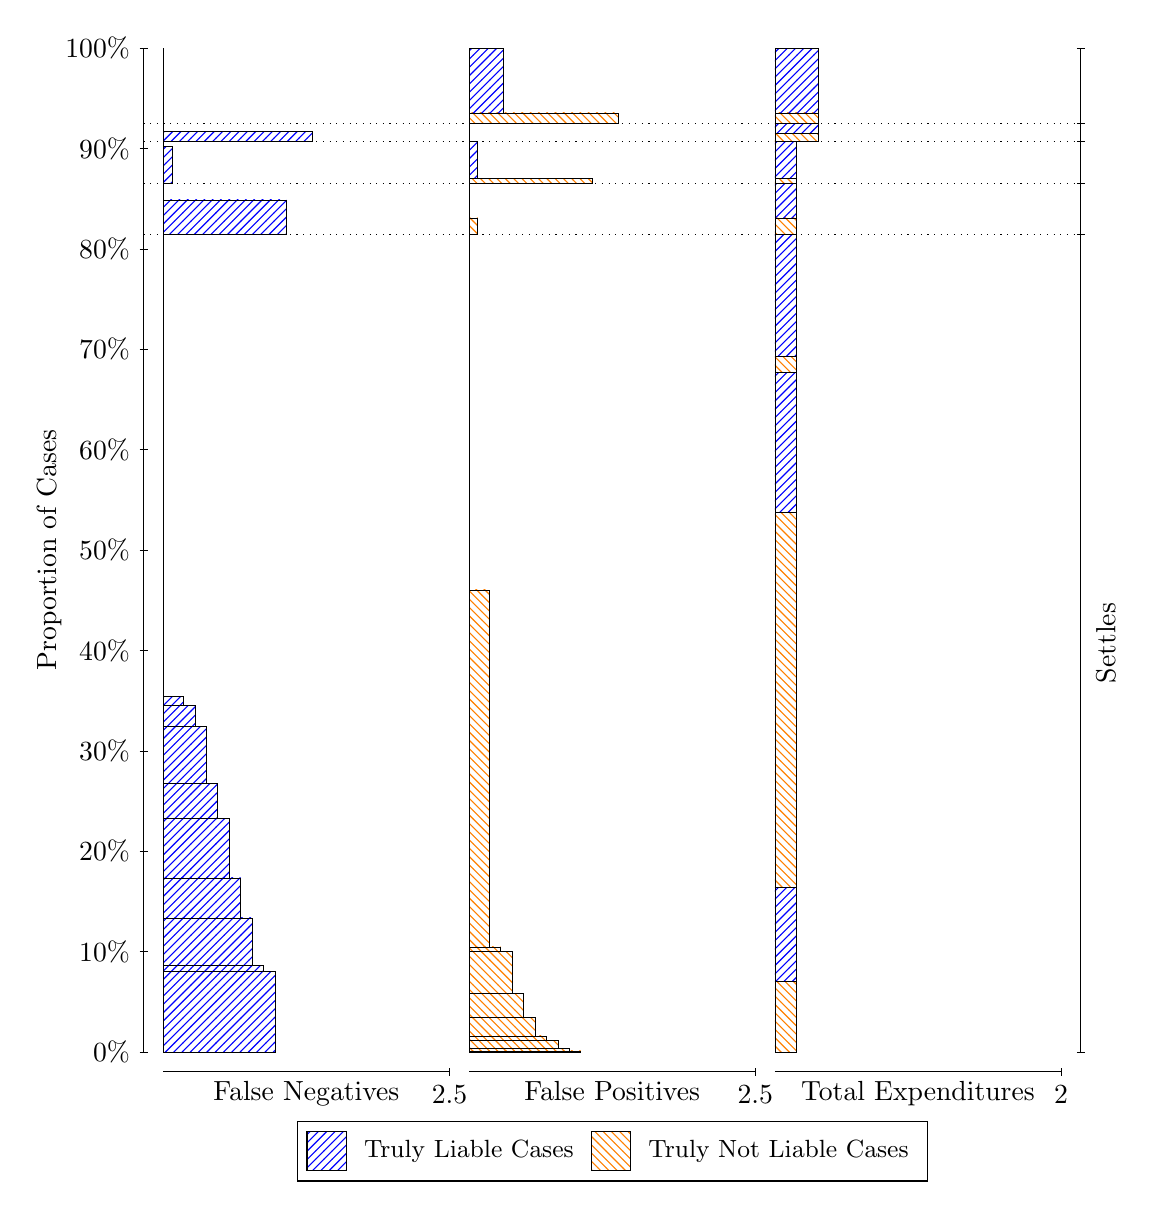
\begin{tikzpicture}
\draw[black, very thin] (1.5,1.75) -- (1.5,14.5);
\node[rotate=90, text=black, anchor=center] at (0.3, 8.125) {Proportion of Cases};
\draw[black, very thin] (1.45,1.75) -- (1.55,1.75);
\node[text=black, anchor=east] at (1.45, 1.75) {0\%};
\draw[black, very thin] (1.45,3.025) -- (1.55,3.025);
\node[text=black, anchor=east] at (1.45, 3.025) {10\%};
\draw[black, very thin] (1.45,4.3) -- (1.55,4.3);
\node[text=black, anchor=east] at (1.45, 4.3) {20\%};
\draw[black, very thin] (1.45,5.575) -- (1.55,5.575);
\node[text=black, anchor=east] at (1.45, 5.575) {30\%};
\draw[black, very thin] (1.45,6.85) -- (1.55,6.85);
\node[text=black, anchor=east] at (1.45, 6.85) {40\%};
\draw[black, very thin] (1.45,8.125) -- (1.55,8.125);
\node[text=black, anchor=east] at (1.45, 8.125) {50\%};
\draw[black, very thin] (1.45,9.4) -- (1.55,9.4);
\node[text=black, anchor=east] at (1.45, 9.4) {60\%};
\draw[black, very thin] (1.45,10.675) -- (1.55,10.675);
\node[text=black, anchor=east] at (1.45, 10.675) {70\%};
\draw[black, very thin] (1.45,11.95) -- (1.55,11.95);
\node[text=black, anchor=east] at (1.45, 11.95) {80\%};
\draw[black, very thin] (1.45,13.225) -- (1.55,13.225);
\node[text=black, anchor=east] at (1.45, 13.225) {90\%};
\draw[black, very thin] (1.45,14.5) -- (1.55,14.5);
\node[text=black, anchor=east] at (1.45, 14.5) {100\%};

\draw[black, very thin] (13.4,1.75) -- (13.4,14.5);
\draw[black, very thin] (13.35,1.75) -- (13.45,1.75);
\node[anchor=west] at (13.35, 1.75) {};
\draw[black, very thin] (13.35,12.136) -- (13.45,12.136);
\node[anchor=west] at (13.35, 12.136) {};
\draw[black, very thin] (13.35,12.779) -- (13.45,12.779);
\node[anchor=west] at (13.35, 12.779) {};
\draw[black, very thin] (13.35,13.318) -- (13.45,13.318);
\node[anchor=west] at (13.35, 13.318) {};
\draw[black, very thin] (13.35,13.547) -- (13.45,13.547);
\node[anchor=west] at (13.35, 13.547) {};
\draw[black, very thin] (13.35,14.5) -- (13.45,14.5);
\node[anchor=west] at (13.35, 14.5) {};

\draw[black, very thin, pattern color=blue, pattern=north east lines] (1.75,1.75) rectangle (3.167,2.7691);
\draw[black, very thin, pattern color=blue, pattern=north east lines] (1.75,2.7691) rectangle (3.0217,2.8466);
\draw[black, very thin, pattern color=blue, pattern=north east lines] (1.75,2.8466) rectangle (2.8763,3.4538);
\draw[black, very thin, pattern color=blue, pattern=north east lines] (1.75,3.4538) rectangle (2.731,3.9623);
\draw[black, very thin, pattern color=blue, pattern=north east lines] (1.75,3.9623) rectangle (2.5857,4.7171);
\draw[black, very thin, pattern color=blue, pattern=north east lines] (1.75,4.7171) rectangle (2.4403,5.1597);
\draw[black, very thin, pattern color=blue, pattern=north east lines] (1.75,5.1597) rectangle (2.295,5.882);
\draw[black, very thin, pattern color=blue, pattern=north east lines] (1.75,5.882) rectangle (2.1497,6.1547);
\draw[black, very thin, pattern color=blue, pattern=north east lines] (1.75,6.1547) rectangle (2.0043,6.269);
\draw[black, very thin, pattern color=orange, pattern=north west lines] (1.75,6.269) rectangle (1.75,12.136);
\draw[black, very thin, pattern color=blue, pattern=north east lines] (1.75,12.136) rectangle (3.3123,12.571);
\draw[black, very thin, pattern color=orange, pattern=north west lines] (1.75,12.571) rectangle (1.75,12.779);
\draw[black, very thin, pattern color=blue, pattern=north east lines] (1.75,12.779) rectangle (1.859,13.25);
\draw[black, very thin, pattern color=orange, pattern=north west lines] (1.75,13.25) rectangle (1.75,13.318);
\draw[black, very thin, pattern color=blue, pattern=north east lines] (1.75,13.318) rectangle (3.6393,13.444);
\draw[black, very thin, pattern color=orange, pattern=north west lines] (1.75,13.444) rectangle (1.75,13.547);
\draw[black, very thin, pattern color=orange, pattern=north west lines] (1.75,13.547) rectangle (1.75,13.676);
\draw[black, very thin, pattern color=blue, pattern=north east lines] (1.75,13.676) rectangle (1.75,14.5);
\draw[black, very thin, pattern color=orange, pattern=north west lines] (5.6333,1.75) rectangle (7.0503,1.764);
\draw[black, very thin, pattern color=orange, pattern=north west lines] (5.6333,1.764) rectangle (6.905,1.7993);
\draw[black, very thin, pattern color=orange, pattern=north west lines] (5.6333,1.7993) rectangle (6.7597,1.8948);
\draw[black, very thin, pattern color=orange, pattern=north west lines] (5.6333,1.8948) rectangle (6.6143,1.9533);
\draw[black, very thin, pattern color=orange, pattern=north west lines] (5.6333,1.9533) rectangle (6.469,2.1854);
\draw[black, very thin, pattern color=orange, pattern=north west lines] (5.6333,2.1854) rectangle (6.3237,2.1935);
\draw[black, very thin, pattern color=orange, pattern=north west lines] (5.6333,2.1935) rectangle (6.3237,2.4954);
\draw[black, very thin, pattern color=orange, pattern=north west lines] (5.6333,2.4954) rectangle (6.1783,3.0239);
\draw[black, very thin, pattern color=orange, pattern=north west lines] (5.6333,3.0239) rectangle (6.033,3.0853);
\draw[black, very thin, pattern color=orange, pattern=north west lines] (5.6333,3.0853) rectangle (5.8877,7.6173);
\draw[black, very thin, pattern color=blue, pattern=north east lines] (5.6333,7.6173) rectangle (5.6333,12.136);
\draw[black, very thin, pattern color=orange, pattern=north west lines] (5.6333,12.136) rectangle (5.7423,12.344);
\draw[black, very thin, pattern color=blue, pattern=north east lines] (5.6333,12.344) rectangle (5.6333,12.779);
\draw[black, very thin, pattern color=orange, pattern=north west lines] (5.6333,12.779) rectangle (7.1957,12.847);
\draw[black, very thin, pattern color=blue, pattern=north east lines] (5.6333,12.847) rectangle (5.7423,13.318);
\draw[black, very thin, pattern color=orange, pattern=north west lines] (5.6333,13.318) rectangle (5.6333,13.42);
\draw[black, very thin, pattern color=blue, pattern=north east lines] (5.6333,13.42) rectangle (5.6333,13.547);
\draw[black, very thin, pattern color=orange, pattern=north west lines] (5.6333,13.547) rectangle (7.5227,13.676);
\draw[black, very thin, pattern color=blue, pattern=north east lines] (5.6333,13.676) rectangle (6.0693,14.5);
\draw[black, very thin, pattern color=orange, pattern=north west lines] (9.5167,1.75) rectangle (9.7892,2.6499);
\draw[black, very thin, pattern color=blue, pattern=north east lines] (9.5167,2.6499) rectangle (9.7892,3.8431);
\draw[black, very thin, pattern color=orange, pattern=north west lines] (9.5167,3.8431) rectangle (9.7892,8.6073);
\draw[black, very thin, pattern color=blue, pattern=north east lines] (9.5167,8.6073) rectangle (9.7892,10.381);
\draw[black, very thin, pattern color=orange, pattern=north west lines] (9.5167,10.381) rectangle (9.7892,10.584);
\draw[black, very thin, pattern color=blue, pattern=north east lines] (9.5167,10.584) rectangle (9.7892,12.136);
\draw[black, very thin, pattern color=orange, pattern=north west lines] (9.5167,12.136) rectangle (9.7892,12.344);
\draw[black, very thin, pattern color=blue, pattern=north east lines] (9.5167,12.344) rectangle (9.7892,12.779);
\draw[black, very thin, pattern color=orange, pattern=north west lines] (9.5167,12.779) rectangle (9.7892,12.847);
\draw[black, very thin, pattern color=blue, pattern=north east lines] (9.5167,12.847) rectangle (9.7892,13.318);
\draw[black, very thin, pattern color=orange, pattern=north west lines] (9.5167,13.318) rectangle (10.062,13.42);
\draw[black, very thin, pattern color=blue, pattern=north east lines] (9.5167,13.42) rectangle (10.062,13.547);
\draw[black, very thin, pattern color=orange, pattern=north west lines] (9.5167,13.547) rectangle (10.062,13.676);
\draw[black, very thin, pattern color=blue, pattern=north east lines] (9.5167,13.676) rectangle (10.062,14.5);
\draw[black, dotted] (1.5,12.136) -- (13.4,12.136);
\draw[black, dotted] (1.5,12.779) -- (13.4,12.779);
\draw[black, dotted] (1.5,13.318) -- (13.4,13.318);
\draw[black, dotted] (1.5,13.547) -- (13.4,13.547);
\draw[black, very thin] (1.75,1.5) -- (5.3833,1.5);
\node[text=black, anchor=north] at (3.5667, 1.5) {False Negatives};
\draw[black, very thin] (5.3833,1.45) -- (5.3833,1.55);
\node[text=black, anchor=north] at (5.3833, 1.45) {2.5};

\draw[black, very thin] (5.6333,1.5) -- (9.2667,1.5);
\node[text=black, anchor=north] at (7.45, 1.5) {False Positives};
\draw[black, very thin] (9.2667,1.45) -- (9.2667,1.55);
\node[text=black, anchor=north] at (9.2667, 1.45) {2.5};

\draw[black, very thin] (9.5167,1.5) -- (13.15,1.5);
\node[text=black, anchor=north] at (11.333, 1.5) {Total Expenditures};
\draw[black, very thin] (13.15,1.45) -- (13.15,1.55);
\node[text=black, anchor=north] at (13.15, 1.45) {2};

\node[text=black, centered, rotate=90] at (13.72, 6.9432) {Settles};





\draw (7.449999999999999,1.5) node[draw=none] (baseCoordinate) {};
\begin{scope}[align=center]
        \matrix[scale=0.5, draw=black, below=0.5cm of baseCoordinate, nodes={draw}, column sep=0.1cm]{
            \node[rectangle, draw, minimum width=0.5cm, minimum height=0.5cm, pattern color=blue, pattern=north east lines] {}; &
            \node[draw=none, font=\small, text=black] (B) {Truly Liable Cases}; &
            \node[rectangle, draw, minimum width=0.5cm, minimum height=0.5cm, pattern color=orange, pattern=north west lines] {}; &
            \node[draw=none, font=\small, text=black] (B) {Truly Not Liable Cases}; \\
            };
\end{scope}

\end{tikzpicture}
\end{document}